% *******************************************************************************
% * Copyright (c) 2007 by Elexis
% * All rights reserved. This document and the accompanying materials
% * are made available under the terms of the Eclipse Public License v1.0
% * which accompanies this distribution, and is available at
% * http://www.eclipse.org/legal/epl-v10.html
% *
% * Contributors:
% *    G. Weirich
% *
% *  $Id: vollversion.tex 4911 2009-01-05 17:56:39Z rgw_ch $
% *******************************************************************************
% !Mode:: "TeX:UTF-8" (encoding info for WinEdt)

\label{vollversion}
\index{version complète}
Si vous avez apprécié la version d'évaluation de Elexis vous de devez en fait rien faire d'autre pour recevoir une version complète : La version d'évaluation \textbf{est} une version complète. La seule différence se trouve dans la base de données.

Pour transformer une version d'évaluation en version complète il faut procéder de façon suivante :
\begin{itemize}
  \item \glqq Installer  \grqq{}le moteur de base de données de la version complète. (\ref{dbengine})
  \item Effacer la base de données de la version d'évaluation (si elle était installée avant).
  \item Lier Elexis avec ce moteur de base de données.  (\ref{connect})
  \item Lier éventuellement avec une version OpenOffice préexistante  \ref{config:ooo}
  \item Introduire la version actuelle des données de base.
  \item Etablir la configuration de base pour votre cabinet médical.

\end{itemize}
Ces pas d'installation ne sont cependant pas si banaux. La mise à jour de l'ensemble des donnés et surtout l'établissement d'un configuration de base convenable pour votre cabinet médical peuvent être assez laborieux. A ce sujet Elexis ne peut pas se distinguer d'autres logiciels de gestion d'un cabinet médical car la complexité de la tâche reste la même pour tous.
Si vous pensez accomplir ce travail vous-même, il faudra réserver suffisamment de temps (une journée au minimum) et suivre ce chapitre étape par étape.
Si vous n'êtes pas sûr de pouvoir le faire nous vous conseillons d' acheter l'installation et la configuration de base y inclus une heure d'instruction pour votre personnel du cabinet.
Ce manuel est par la force des choses un peu penché sur la Suisse. Pour d'autre pays probablement pas toutes les informations sont correctes respectivement utiles.
\bigskip

Pour compléter nous attirons votre attention sur le fait que cette documentation peut contenir des fautes et pourrait être incomplète. Nous ne pouvons pas assumer la responsabilité si vous subissez des dégâts matériels ou immatériels suite à une configuration défectueuse ou une documentation incorrecte. Nous vous conseillons de minutieusement tester le tout et si possible aussi de faire des contrôles manuels (par exemple des factures) avant de travailler \glqq véritablement \grqq{} avec votre configuration. 

\section{Ce dont vous avez besoin}
Avant de commencer la configuration vous devez collectionner les programmes et données suivants :
\begin{itemize}
  \item Kit d'installation pour votre serveur de base de données
  \item Noms, Noms d'utilisateur et mots de passe pour tous qui devaient pouvoir utiliser Elexis
  \item Noms, Numéros du Concordat , Numéros EAN, Coordonnées bancaires ou pour le compte de chèque postal, numéros de participant BVR de tous les mandants.
  \item Relevé actualisé des valeurs du point de votre canton
  \item Une conception de vos en-têtes pour lettres, ordonnances, certificats.
  \item Une liste des examens de laboratoire effectués dans votre laboratoire du cabinet.
  \item Liste des médicaments, CIM-10, Tarmed , Liste des analyses, MiGel dans la mesure où vous en avez besoin.
  \item Les numéros EAN des assurances maladies et accidents
\end{itemize}

\section{Installation du moteur de base de données}
\label{dbengine}
L'installation de Elexis consiste en deux parties : Un \textit{Serveur} sur lequel sont installés les données et un ou plusieurs \textit{Clients}, qui ont accès aux données et qui permettent de les visualiser et de les modifier. Le serveur et les clients peuvent se trouver sur le même ou sur des différents ordinateurs.
Un\textit{\textit{Serveur}} au sens large est un ordinateur à part sur lequel fonctionnent un ou plusieurs logiciels serveur.

Elexis peut utiliser (en principe une quelconque) base de données qui se laisse utiliser selon le standard de l'industrie JBBC comme logiciel de serveur. L'installation automatique est configurée d'avance pour les systèmes de base de données suivants :
\begin{itemize}
\item MySQL (\href{http://www.mysql.com}{www.mysql.com}): Il s'agit de la base de données le plus répandue dans l'Internet. La majorité des applications basées sur une base de données qu'on trouve dans le Web, utilisent en arrière-plan un serveur MySQL. Un serveur MySQL coute environs Fr 750.-pour une utilisation à des fins commerciales. A des fins privés il est gratuit.

\item PostgreSQL (\href{http://www.postgresql.org}{www.postgresql.org}): Il s'agit d'un serveur de base de données OpenSource. Il maîtrise un jeu d'instructions plus large que MySQL mais est considéré comme un peu plus lent que celui-ci. Cependant cela ne devrait pas jouer un rôle pour Elexis car les test de rapidité se font normalement sous les conditions de plusieurs milliers d'accès par seconde, un situation qui pourrait se produire que dans des très rares cas dans un cabinet médical. PostgreSQL est gratuit pour toutes les formes d'utilisation.

\item HSQLDB: Il s'agit d'une base de données OpenSource qui est écrite en Java. Elle peut être utilisée soit en tant que serveur indépendant soit intégrée dans le logiciel. HSQL est un peu plus lent que les deux systèmes mentionnés précédemment mais pour des environnements petits comme ceux d'un cabinet médical éventuellement suffisant. Cependant il faut faire spécifiquement attention en ce qui concerne la sauvegarde des données car une panne d'ordinateur (ou même le fait d'éteindre l'ordinateur de façon improviste) peut rendre la base de données inutilisable. HSQL est gratuit.
\end{itemize}

\textbf{Attention}: Nous \textit{déconseillons explicitement} l'utilisation du serveur de base de donnée HSQL utilisé pour la version d'évaluation de Elexis pour le travail au cabinet médical (risque de perte des données !) Nous vous conseillons plutôt d'installer MySQL ou PostgreSQL.
\begin{itemize}
 \item Comme serveur nous vous conseillons de choisir de préférence un ordinateur sur lequel personne ne travaille directement. Qu'il y ait encore d'autres logiciels de serveur installés comme par ex. pour les mails, fax, imprimantes etc, ne joue aucun rôle. Attention! Si vous n'installez pas le serveur de base de donnée sur un ordinateur réservé à cette fonction mais sur un poste de travail il doit avoir au moins 1 GB de RAM et 2 GB seraient préférable.
 \item Installez là le serveur de base de donné de votre choix. (Nous préconisons mysql ou PostgreSQL)
 \item Créez dans la base de donnée un 'user-account' nommé : elexisuser
 \item Créez une base de donnée (vide) avec le nom elexis sur laquelle 'elexisuser' a un accès illimité.
 \item Décidez-vous absolument pour une stratégie de sauvegarde des données efficace et fiable. Plus d'information la concernant ci-après.
 \item La configuration ultérieure se fait depuis les 'clients'. Pour le travail de tout les jours le serveur ne nécessite pas forcément un écran et un clavier et peut se trouver à un endroit frais du cabinet ou même à la cave.
\end{itemize}

\textbf{Important!}
\textit{N'oubliez jamais la sauvegarde des données!}

Elexis enregistre toutes les données dans cette base des données. Une destruction de cette base de donnée n'est pas du tout impossible. Une interruption du courrant peut \glqq  choper le disque dur au tendon d'Achille\grqq{} un dommage mécanique peut détruire des secteurs importants du disque dur et les rendre illisibles, une faute d'un logiciel peut effacer les données et un virus peut se défouler sur vos données. Il y a des multiples stratégies de sauvegarde des données. Nous vous présenterons quelques unes en ce qui suit :

\begin{description}
\item[ La Réplication  ] Certaines banques de données (comme par exemple MySQL à partir de la version 4.0) peuvent copier leurs données de façon constante vers un serveur qui se trouve sur un autre ordinateur. Puisque seulement les données qui changent sont transmis (en arrière-plan) ceci demande moins de capacité que ce qu'on pourrait croire. Cette méthode s'appelle la  \textit{Réplication} . En fin de compte on a deux bases de données identiques. Si le serveur se casse on peut dans un délai de quelques minutes choisir le deuxième ordinateur comme serveur et continuer le travail pratiquement sans interruption.
\item [La Machine virtuelle ] Un concept apparenté : On laisse tourner le serveur de la base de donnée sur un machine virtuelle spécifiquement réservée pour cela (par ex. de VMWare) et on sauvegarde de façon régulière toute la machine virtuelle. En cas de panne du serveur on peut également dans quelques minutes starter la machine virtuelle de sauvegarde sur le même ou n'importe quel autre ordinateur dans le réseau et continuer à travailler.
\item [Sauvegarde des données fréquente ] On peut laisser faire toutes les quelques minutes une sauvegarde automatisée (par ex. avec mysqldump) et sauvegarder de cette façon des données en plusieurs générations sur des différents supports informatiques. Cette méthode utilise le moins de ressources de toutes les méthodes mentionnées ici et crée les fichiers de sauvegarde les plus petits. En cas de panne du serveur par contre la remise en route prend plus de temps : Il faut d'abord démarrer le serveur de base de donnée sur un ordinateur de réserve et y mettre les fichiers sauvegardés pour ensuite adapter selon la configuration tout les 'clients' au nouveau serveur.
\end{description}

\section{Effacer la base de donnée de la version d'évaluation}
Si Elexis trouve lors du démarrage une base de donnée de la version d'évaluation le lien sera toujours fait avec cette base de donnée indépendamment des réglages de connexion que vous avez défini. Pour cette raison vous devez d'abord fermer Elexis et effacer ou renommer la base de donnée de la version d'évaluation qui se trouve dans le répertoire  \glqq demoDB\grqq{}dans le répertoire du programme Elexis. Après avoir effacé ou renommé ce répertoire vous pouvez redémarrer Elexis qui devrait être maintenant apte à se connecter à votre nouvelle base de donnée que vous avez installé préalablement.

\section{Créer un lien avec la base de données}
\label{connect}
Démarrez Elexis et choisissez dans le menu  Fichier -> Connexion.

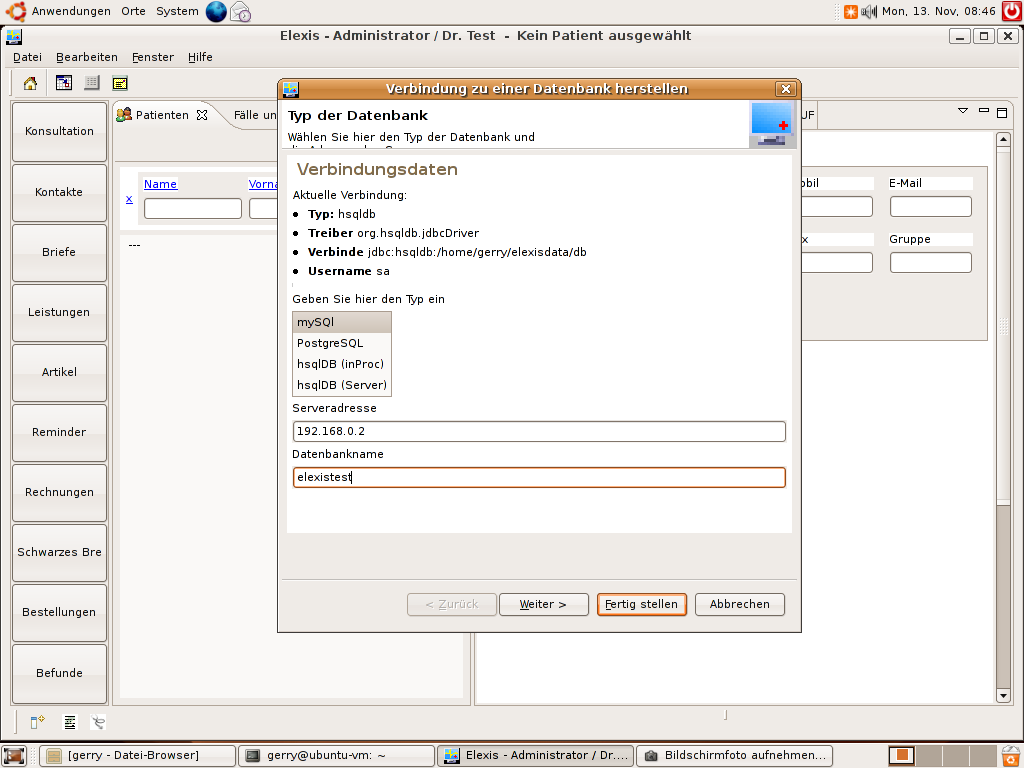
\includegraphics[width=0.9\textwidth]{images/verbindung11.png}
% verbindung11.png: 1024x768 pixel, 72dpi, 36.12x27.09 cm, bb=0 0 1024 768



Entrez le type de base de donnée (ici mysql), l'adresse du serveur (ici 192.168.0.2) ou son nom Internet (par ex. testserver.elexus.ch) de même que le nom de la base de donnée (ici elexistest) et cliquez sur
\textit{suite}.

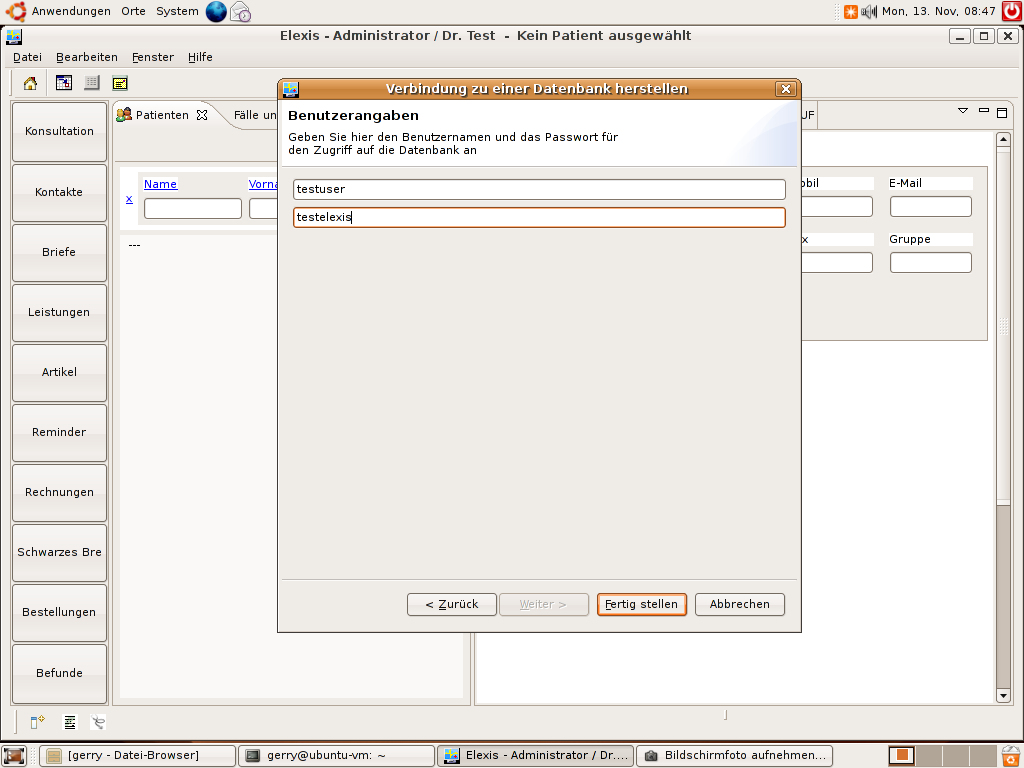
\includegraphics[width=0.9\textwidth]{images/verbindung12.png}
% verbindung12.png: 1024x768 pixel, 72dpi, 36.12x27.09 cm, bb=0 0 1024 768
Introduisez dans la ligne supérieure le nom d'utilisateur pour la base de donnée (ici testuser) et dans la ligne inférieure le mot de passe (ici testelexis) et cliquez sur \textit{terminer}.

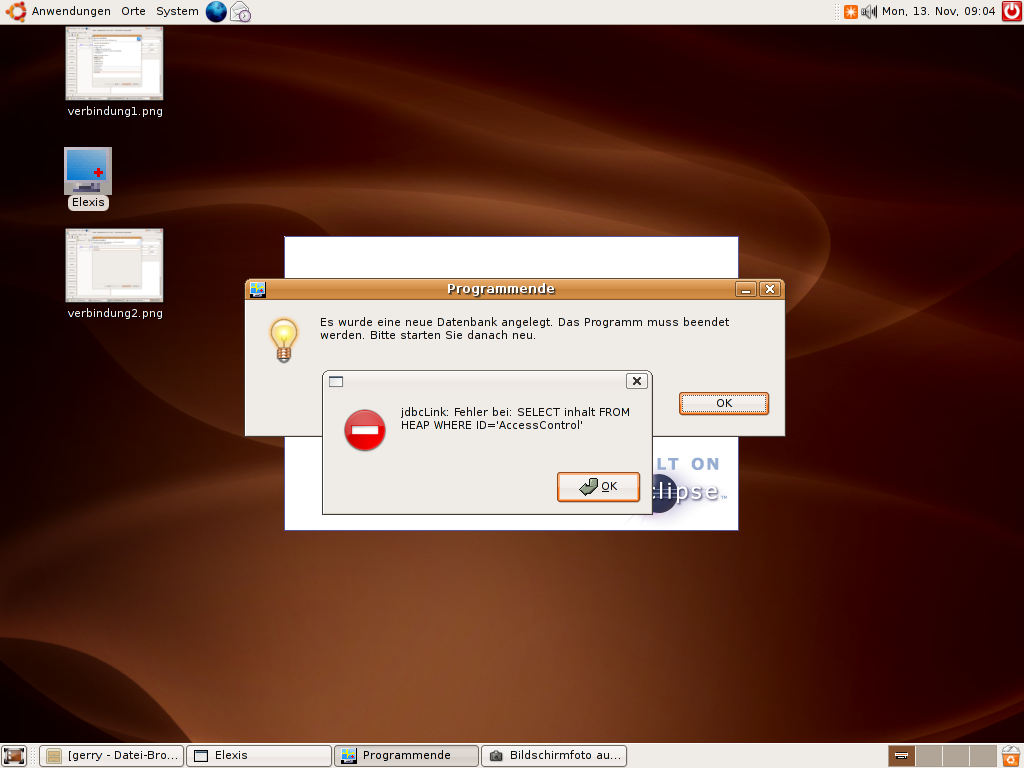
\includegraphics[width=0.9\textwidth]{images/verbindung13.png}
% verbindung13.png: 1024x768 pixel, 72dpi, 36.12x27.09 cm, bb=0 0 1024 768

Il y aura quelques messages d'erreur qui apparaîtront mais vous pouvez les ignorer en les fermant. Enfin il faut redémarrer Elexis.

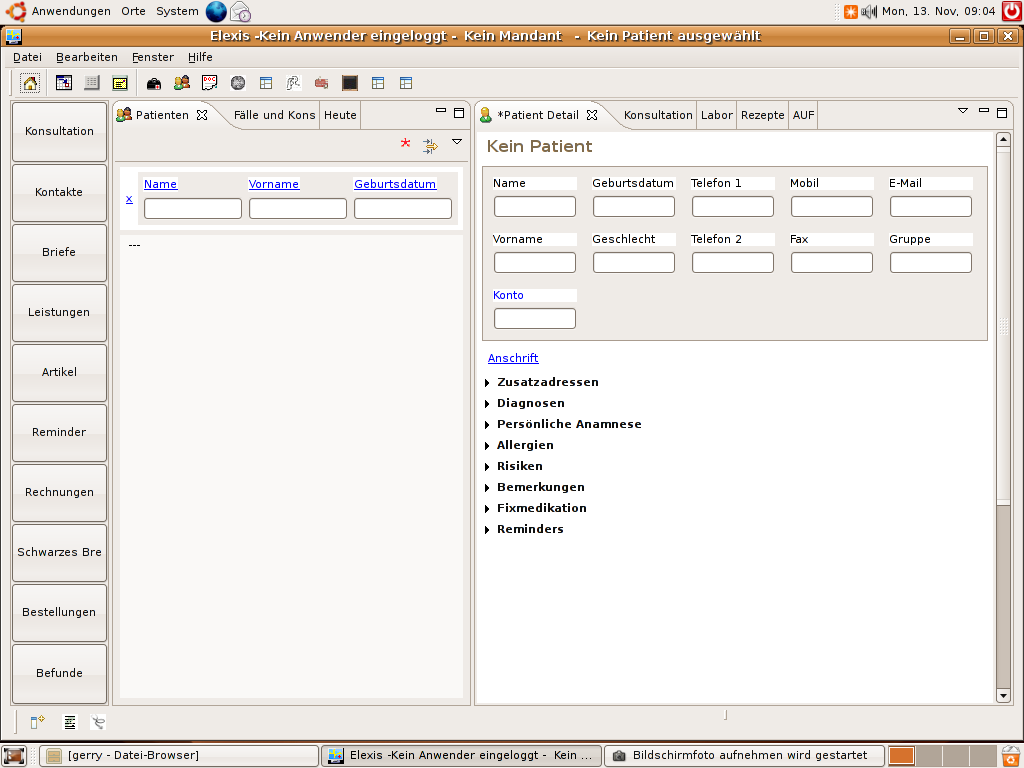
\includegraphics[width=4in]{images/verbindung14.png}
% verbindung14.png: 1024x768 pixel, 72dpi, 36.12x27.09 cm, bb=0 0 1024 768

Vous pouvez maintenant faire une login dans le nouveau système Elexis avec le nom \textit{Administrator} et le mot de pass \textit{admin}.

\section{Lier avec Open-Office}
\label{config:ooo}
Le fichier d'installation contient déjà une version complète de OpenOffice. Si vous voulez travailler avec celle-ci vous ne devez faire rien de plus. 
Si vous avez par contre déjà installé une autre version de OpenOffice sur votre ordinateur, la version apportée par Elexis pourrait provoquer des conflits. Procédez en ce cas là de façon suivante :


\begin{itemize}
\item Effacez le répertoire ooo dans le répertoire de Elexis (ou renommez-le).
\item Redémarrez Elexis
\item Allez sous  \textsc{Fichier - Options - NOAText} cliquez sur \glqq définir\grqq{} et choisissez le répertoire de l'installation existante de OpenOffice et cliquez sur \textit{appliquer}.

\end{itemize}
\section{Entrer les données de base}
\subsection{Tarmed}
\index{Tarmed}
Vous pouvez télécharger une base de donnée Microsoft Access depuis www.tarmedsuisse.ch
Intégrez cette base de donnée dans votre PC avec système d'exploitation Windows comme DSN système. Choisissez dans Elexis \textit{WINDOW - PESPECTIVE - OTHER - PRESTATIONS}. Sous \textit{Codes}, vous trouverez un onglet  \textit{Tarmed}. Dans le 'View-menu' (petit triangle en haut à droite) vous choisissez \textit{import} et introduisez la base de donnée que vous venez d'intégrer comme DNS système. Dépendant de la vitesse de l'ordinateur l'importation de toute la base de donnée Tarmed prendra entre une à 5 minutes.

\subsection{CIM-10 (ICD-10)}
\index{CIM-10 (ICD-10)}
\label{config:icd10}
Vous pouvez télécharger le catalogue CIM-10 de l'OMS en forme informatisée de:

http://www.icd10.ch/index.asp

Vous avez besoin de la \textit{version informatisée ASCII de la CIM-10 systématique de l'OMS } et des \textit{métadonnées systématiques 2006 de la CIM-10 de l'OMS ASCII}. Décompressez tout les deux fichiers zip dans le même dossier. Vous pouvez ignorer l'avertissement que vous êtes en train d'écraser un fichier. Choisissez dans Elexis  WINDOW - PERSPECTIVE - OTHER - PRESTATIONS. Sous 'Codes' vous trouverez un onglet \textit{CIM-10}. Dans le 'View-menu' (petit triangle en haut à droite) vous choisissez  \textit{import}. et introduisez le dossier dans lequel vous avez décompressé les deux fichiers.

\subsection{Médicaments et Medicals}
\index{médicaments}\index{Medicals}\index{SL}
Ces deux groupes ont l'origine dans la même base de donnée. Vous nécessitez la liste transfer.dat que vous pouvez abonner par exemple chez www.e-mediat.ch. Choisissez dans Elexis 'WINDOW - PERSPECTIVE - OTHER - ARTICLES'. Sous 'Articles' vous trouverez les onglets \textit{Medicals} respectivement \textit{Médicaments}. Dans le 'View-menu' (petit triangle en haut  à droite) vous choisissez 'import' et introduisez le chemin d'accès pour le dossier dans lequel vous avez mis le fichier Transfer.dat.

\subsection{Liste des analyses}
\index{Liste des analyses}\index{LA}\index{LFA}
Cette liste est publiée par l'OFSP et actuellement pour des raisons incompréhensibles seulement en format pdf. Ceci nous force de faire en plus un pas de conversion qui risque certaines fautes de transcription. Sous Windows c'est le logiciel TextFromPDF qui est capable de faire la conversion, sous Linux par exemple xpdf. Veuillez constituer par ces logiciels une version plaintext de la liste des analyses. Ensuite vous procédez de nouveau dans Elexis 'WINDOW - PERSPECTIVE - OTHER - PRESTATIONS'. Sous \textit{Codes} vous trouverez l'onglet 'Analyses'. Dans le 'View-menu' (petit triangle en haut à droite) vous choisissez 'import' et introduisez le chemin d'accès pour le dossier dans lequel vous avez mis le fichier converti de la liste des analyses.
\subsection{LiMA}
\index{LiMA}
La liste LiMA n'est fourni par l'OFSP, une fois de plus, qu'en format pdf de sorte qu'on doive d'abord péniblement déboîter le ficher pour faire ensuite une conversion . Pour cela vous utilisez de nouveau sous Windows le logiciel TextFromPDF, sous Linux par exemple xpdf. Puisque la structure n'est pas si facilement automatiquement analysable comme c'était le cas avec la liste des analyses, vous devez faire en plus un pas supplémentaire. Le fichier texte doit être transformé en tableau au format .csv qui contient les colonnes : code, texte, unité, prix. Pour cette transformation vous pouvez utiliser par exemple OpenOffice Calc ou Microsoft Excel. Ensuite vous procédez de nouveau dans Elexis 'WINDOW - PERSPECTIVE - OTHER - ARTICLES'. Sous 'ARTICLES' vous trouverez l'onglet \textit {MiGel = LiMA}. Dans le 'View-menu' (petit triangle en haut à droite) vous choisissez \textit{import} et introduisez le chemin d'accès pour le dossier dans lequel vous avez mis le fichier converti de la liste LiMA.

\section{Configuration de base}
\index{Configuration de base}
\label{grundkonfiguration}
La configuration de base se fait par les pas suivants :
\begin{itemize}
  \item Installer les mandants et utilisateurs
  \item Définir les paramètres du laboratoire
  \item Créer des modèles de texte
  \item Installer le module de facturation
\end{itemize}
\subsection{Installer les mandants et les utilisateurs}
Ouvrez la perspective \textit{Contacts},

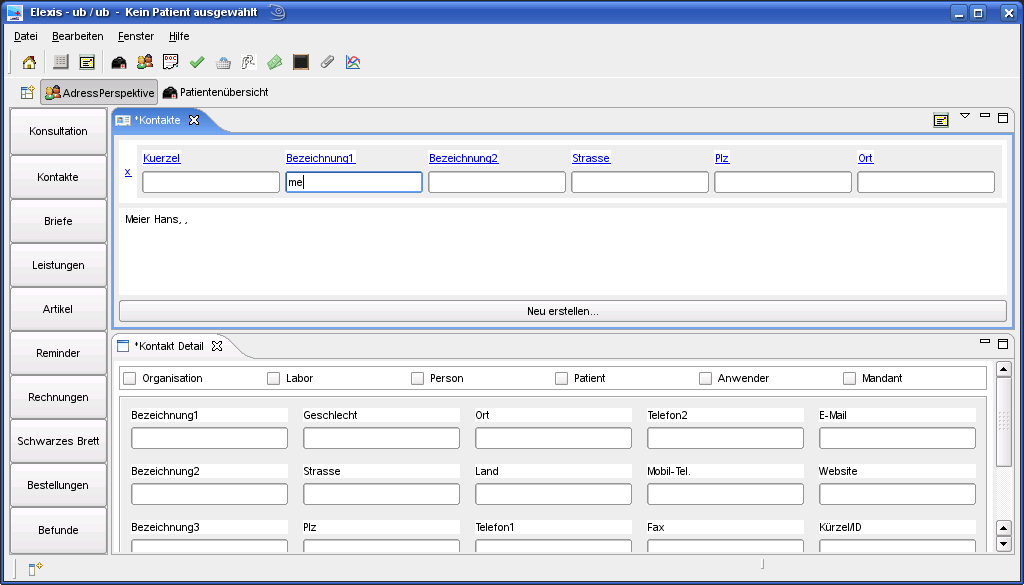
\includegraphics[width=4.5in]{images/grundkonfkonta.png}
% grundkonfkonta.png: 1024x585 pixel, 72dpi, 36.12x20.64 cm, bb=0 0 1024 585
\begin{itemize}
 \item Introduisez sous \textit{Bezeichnung1 = désignation1} le nom du nouveau mandant ou du nouvel utilisateur et cliquez sur \textit{créer nouveau}.
 \item Cliquez ensuite sur l'entrée que vous venez d'introduire dans la liste en haut de la page et complétez les données dans la partie inférieure. Comme toujours chez Elexis, il n'est pas indispensable de remplir toujours tous les champs. Ensuite vous \textit{déterminez} si le contact introduit sera  \textit{mandant} ou \textit{utilisateur} (Un mandant est toujours aussi un utilisateur et les deux sont toujours des \textit{personnes}
 \item Lorsque vous avez introduit tout les mandants et utilisateurs, vous allez sous 'Fichier - Options' et vous trouverez sous 'groupes, droits et accès' l'onglet \textit{mandant}
\end{itemize}

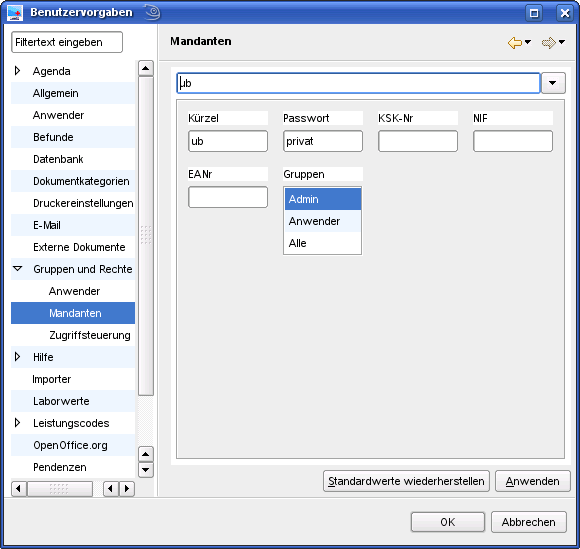
\includegraphics[width=4in]{images/grundkonfmand.png}
% grundkonfmand.png: 580x549 pixel, 72dpi, 20.46x19.37 cm, bb=0 0 580 549
\begin{itemize}
 \item Introduisez les données nécessaires pour les mandants déjà installés. Introduisez comme  \textit{sigle} le nom d'utilisateur et comme mot de passe le mot de passe attribué au mandant. Tout le reste dépend du type du mandant.

 \item Ensuite vous allez sous 'Sécurité' - utilisateurs
\end{itemize}

Introduisez là pour tout les \index{utilisateurs}utilisateurs définis les données respectives. N'oubliez pas de définir (sous utilisateur) pour chaque utilisateur un mandant de référence  (\textit{pour mandant}). Un mandant de référence (normalement lui-même) devrait être établi aussi pour des mandants déjà introduits (que vous trouvez aussi sous "utilisateurs" car un mandant est toujours aussi un utilisateur). Le mandant de référence définit pour qui l'utilisateur travaille normalement. Ceci peut être changé pendant le travail (sous  \textit{Fichier - Mandant}...),mais lors du login tout d'abord c'est le mandant de référence qui est activé.

\subsection{Introduire les paramètres du laboratoire}
Ouvrez d'abord de nouveau le \textit{View-Contacts}. Introduisez là votre laboratoire interne et aussi le laboratoire externe et marquez-les comme \textit{Laboratoire}
%TODO!!

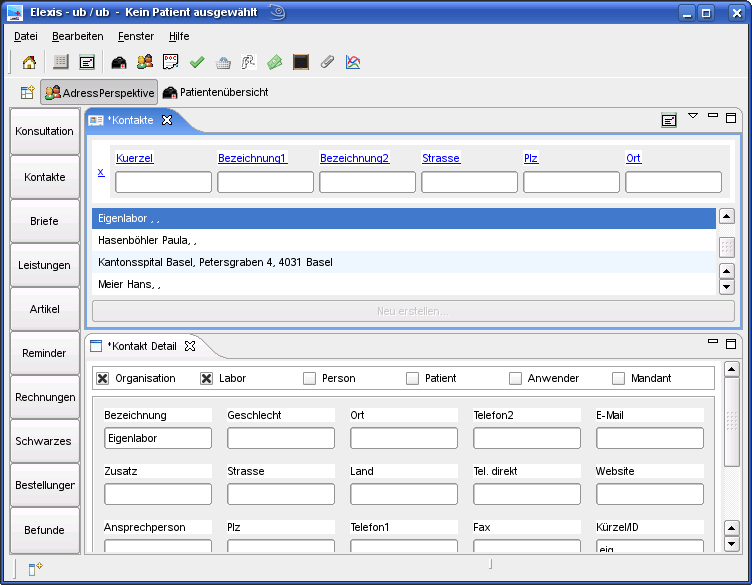
\includegraphics[width=4in]{images/grundkonfmand1.png}
% grundkonfmand1.png: 752x585 pixel, 72dpi, 26.53x20.64 cm, bb=0 0 752 585

\subsection{Configurer le programme de texte}

Elexis travaille jusqu'alors que avec OpenOffice, raison pour laquelle nous expliquons ici que la configuration avec OpenOffic.

\begin{itemize}
 \item Si vous ne l'avez pas encore fait, installez OpenOffice (au minimum version 2.0)
 \item Choisissez dans Elexis sous \textit{Fichier - Options - Traitement de texte 1 : NOA-Text}
\end{itemize}

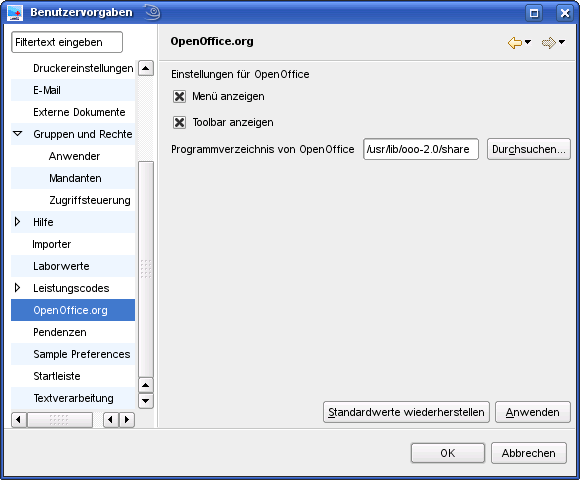
\includegraphics[width=3.5in]{images/grundkonfmand2.png}
% grundkonfmand2.png: 580x480 pixel, 72dpi, 20.46x16.93 cm, bb=0 0 580 480

\begin{itemize}
 \item Allez dans Elexis sous  \textit{Fichier - Options sous OpenOffice} et cherchez le chemin d'accès du sous répertoire 'program' de l'installation OpenOffice. Pour ceci vous cliquez sur 'Define = définir' et choisissez sous 'browse' le sous répertoire. Il se trouve sous Windows normalement sous : C./progammes/OpenOffice.org 2.0/programme respectivement à l'endroit où vous l'avez installé.
 \item Cliquez sur \textit{Apply=appliquer}, fermez la configuration et redémarrez Elexis. 
 \item Si vous ouvrez par ex. la 'Perspective - Lettres', la fenêtre de OpenOffice devrait s'ouvrir dans la fenêtre de Elexis. (Ceci durera lors de la première utilisation assez long temps ~30 secondes).
\end{itemize}

\subsubsection{\index{modèles!Druckvorlagen}Créer un modèle}
Pour quelques formulaires Elexis cherche des modèles prédéfinis qui ont un nom spécifique. Ces modèles définissent pour certains formulaires l'apparence spécifique pour leur fonction. Pour des données variables il faudra y introduire à des endroits spécifiques des espaces réservés.
Pour créer un formulaire vous procédez de la façon suivante :
Préparez votre formulaire tout normalement dans le programme de traitement de texte et sauvegardez-le comme tout document avec texte. Depuis Elexis vous choisissez la perspective \textit{Lettres} et ensuite 

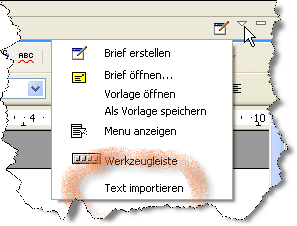
\includegraphics[width=2.5in]{images/import.png}
% import.png: 297x226 pixel, 96dpi, 7.86x5.98 cm, bb=0 0 223 169

le View-menu à droite.

Choisissez là  \textit{Text importer} et cherchez le formulaire que vous venez de créer. Par cette action vous importez le document dans Elexis. Ensuite vous pouvez encore faire des adaptation du texte et après avoir fini vous choisissez de nouveau le View-menu à droite. Cette fois-ci vous choisissez \textit{sauvegarder comme modèle}.

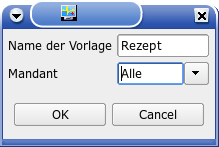
\includegraphics[width=2.5in]{images/rezept1.png}
% rezept1.png: 219x147 pixel, 72dpi, 7.73x5.19 cm, bb=0 0 219 147

 Comme\textit{nom du modèle} vous devez introduire pour les modèles standard mentionnés en bas la nom correspondant pour des modèles personnels vous pouvez par contre utiliser des désignations quelconques. Sous  \textit{mandant} vous pouvez définir pour quel mandant ce modèle avait été crée ou si tout le monde l'utilisera.
 
Figurant ci-dessous vous trouvez une liste des modèles standard :


\begin{itemize}
\item Ordonnance : \index{modèles!ordonnance}Vous avez besoin pour cela un modèle nommé \textit{ordonnance}. Il pourrait se voir par exemple de cette façon :
 \end{itemize}
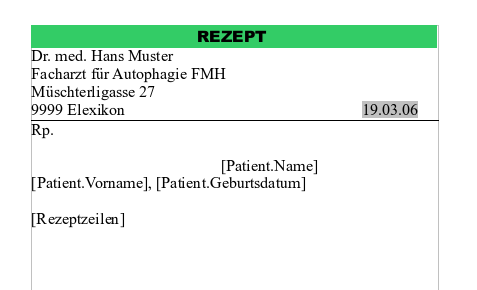
\includegraphics[width=4in]{images/rezept.png}
% rezept.png: 477x290 pixel, 72dpi, 16.83x10.23 cm, bb=0 0 477 290

A l'endroit où c'est écrit  [Rezeptzeilen] vous introduirez plus tard les médicaments que vous choisissez. Cette variable est donc indispensable. Tout les autres éléments du modèle \textit{ordonnance} sont facultatifs.

\begin{itemize}
 \item \textit{Certificat d'incapacité de travail }: Un modèle pour le certificat d'incapacité de travail.  Vous pouvez introduire comme variable[AUF.Grund=raison d'incapacité], [AUF.von=incapacité de ...], [AUF.bis=incapacité à ...], [AUF.Prozent=incapacité pourcentage] et tout les variables standards . Tous sont facultatives.


 \item \textit{Feuille labo}: Pour imprimer les résultats du laboratoire. Les résultats sont introduits dans la variable  Laborwerte  et cette variable est indispensable, d'autres peuvent être introduites selon besoin. 
 \item \textit{Liste}: Il s'agit de l'impression des différentes données en forme de listes. Quelque part doit se trouver la variable  Liste  à laquelle peuvent être jointes les données.


\end{itemize}

Des Plugins que vous utilisez peuvent éventuellement nécessiter certains modèles.

\subsection{Installer le module de facturation}
\label{conf:abrechnung}
Il est indispensable que l'installation de ce module soit fait avant de vouloir introduire des prestations. Le procédé dépend du module de facturation. Pour le module des tarifs pour les médecins en Suisse le procédé est décrit lors de la description du Plugin correspondant sous (S. \ref{arzttarife}, page \pageref{arzttarife} ff.)

